\documentclass[11pt]{article}

% ---------- Page layout ----------
\usepackage[a4paper, margin=2.2cm, headheight=14pt]{geometry}
\usepackage{setspace}
\setstretch{1.08}
\setlength{\parskip}{0.45em}
\setlength{\parindent}{0pt}

% ---------- Math (load before fonts) ----------
\usepackage{amsmath,amsthm}

% ---------- Fonts ----------
\usepackage[T1]{fontenc}
\usepackage[utf8]{inputenc}
\usepackage{newtxtext,newtxmath}   % Times-style text and math; already includes amssymb symbols
\usepackage{microtype}

% ---------- Figures and tables ----------
\usepackage{graphicx}
\usepackage{booktabs}
\usepackage{caption}
\captionsetup{font=small, labelfont=bf}
\usepackage{dsfont}   % \mathds{1}: newtxmath has no blackboard-bold digits
\usepackage{pifont}   % \ding check and cross marks
\usepackage{tikz}
\usetikzlibrary{arrows.meta,decorations.pathreplacing}

% ---------- Figure colors ----------
\definecolor{bgPrimary}{HTML}{DAE8FC}
\definecolor{bgAccent}{HTML}{B3CDE3}
\definecolor{borderPrimary}{HTML}{6C8EBF}
\definecolor{borderAccent}{HTML}{3A6EA5}
\definecolor{arrowColor}{HTML}{4A6A8A}
\definecolor{textMain}{HTML}{2C3E50}
\definecolor{textLight}{HTML}{7F8C8D}
\definecolor{bgHighlight}{HTML}{FFF3CD}
\definecolor{borderTarget}{HTML}{C9A227}
\definecolor{okBorder}{HTML}{5B9F6E}
\definecolor{badBorder}{HTML}{C0605A}

% ---------- Section style ----------
\usepackage{titlesec}
\titleformat{\section}
  {\Large\bfseries}{\thesection}{0.8em}{}
  % [{\titlerule[0.5pt]}]
\titleformat{\subsection}
  {\large\bfseries}{\thesubsection}{0.6em}{}
\titleformat{\subsubsection}
  {\normalsize\bfseries}{\thesubsubsection}{0.5em}{}
\titlespacing*{\section}{0pt}{1.4em}{0.8em}
\titlespacing*{\subsection}{0pt}{1.1em}{0.5em}

% ---------- Header and footer ----------
\usepackage{fancyhdr}
\pagestyle{fancy}
\fancyhf{}
\fancyhead[L]{\small\itshape Scaling Verification Depth for Stronger Reasoning}
\fancyhead[R]{\small\itshape October 2026}
\fancyfoot[C]{\small\thepage}
\renewcommand{\headrulewidth}{0.4pt}

% ---------- References and links ----------
\usepackage[numbers]{natbib}
\usepackage[hidelinks]{hyperref}
\usepackage[capitalise]{cleveref}

% ---------- Theorem environments ----------
\theoremstyle{definition}
\newtheorem{definition}{Definition}
\theoremstyle{plain}
\newtheorem{proposition}{Proposition}

% ---------- Title block ----------
\makeatletter
\renewcommand{\maketitle}{%
  \thispagestyle{plain}
  \begin{center}
    \rule{\linewidth}{1.2pt}\par\vspace{0.9em}
    {\LARGE\bfseries\@title\par}\vspace{0.7em}
    {\large\@author\par}\vspace{0.25em}
    {\small\@date\par}\vspace{0.6em}
    % \rule{\linewidth}{0.5pt}
  \end{center}
  \vspace{1em}
}
\makeatother

\title{Scaling Verification Depth for Stronger Reasoning}
\author{Tue Le}
\date{October 2026}

\begin{document}

\maketitle

\begin{center}
\captionsetup{type=figure}
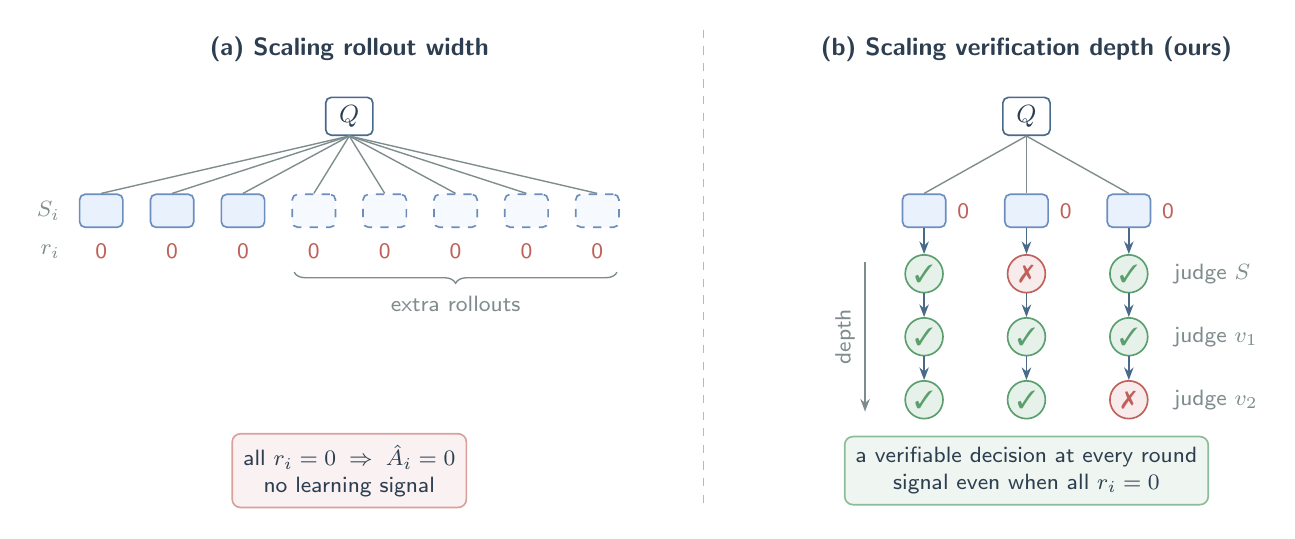
\begin{tikzpicture}[
  x=1cm, y=1cm,
  font=\sffamily\small,
  every node/.style={text=textMain},
  >={Stealth[length=1.6mm]},
  qn/.style={rounded corners=2pt, draw=arrowColor, fill=white, line width=0.6pt, minimum width=0.6cm, minimum height=0.48cm, inner sep=1pt},
  sol/.style={rounded corners=2pt, draw=borderPrimary, fill=bgPrimary!60, line width=0.6pt, minimum width=0.55cm, minimum height=0.42cm, inner sep=1pt},
  extra/.style={sol, dashed, fill=bgPrimary!25},
  ok/.style={circle, draw=okBorder, fill=okBorder!15, line width=0.6pt, minimum size=0.48cm, inner sep=0pt, text=okBorder, node contents=\ding{51}},
  bad/.style={circle, draw=badBorder, fill=badBorder!12, line width=0.6pt, minimum size=0.48cm, inner sep=0pt, text=badBorder, node contents=\ding{55}},
  edge/.style={draw=textLight, line width=0.5pt},
  flow/.style={->, draw=arrowColor, line width=0.6pt},
  lab/.style={font=\sffamily\footnotesize, text=textLight},
  ttl/.style={font=\sffamily\small\bfseries},
  msg/.style={rounded corners=3pt, line width=0.6pt, align=center, inner sep=4pt, font=\sffamily\footnotesize},
]
% ---------- (a) Rollout width ----------
\node[ttl] at (3.8,0.85) {(a) Scaling rollout width};
\node[qn] (qa) at (3.8,0) {$Q$};
\foreach \j in {1,...,8} {
  \pgfmathsetmacro{\x}{0.65+0.9*(\j-1)}
  \ifnum\j<4 \node[sol] (a\j) at (\x,-1.2) {};
  \else      \node[extra] (a\j) at (\x,-1.2) {};
  \fi
  \draw[edge] (qa.south) -- (a\j.north);
  \node[font=\sffamily\footnotesize, text=badBorder] at (\x,-1.72) {0};
}
\node[lab, anchor=east] at (0.25,-1.2)  {$S_i$};
\node[lab, anchor=east] at (0.25,-1.72) {$r_i$};
\draw[textLight, line width=0.5pt, decorate, decoration={brace, amplitude=4pt, mirror}]
  (3.1,-1.98) -- (7.2,-1.98);
\node[lab] at (5.15,-2.38) {extra rollouts};
\node[msg, draw=badBorder!60, fill=badBorder!8] at (3.8,-4.5)
  {all $r_i=0\;\Rightarrow\;\hat A_i=0$\\no learning signal};

\draw[textLight!60, dashed] (8.3,1.1) -- (8.3,-5.0);

% ---------- (b) Verification depth ----------
\node[ttl] at (12.4,0.85) {(b) Scaling verification depth (ours)};
\node[qn] (qb) at (12.4,0) {$Q$};
\foreach \s/\x/\ra/\rb/\rc in {1/11.1/ok/ok/ok, 2/12.4/bad/ok/ok, 3/13.7/ok/ok/bad} {
  \node[sol] (b\s) at (\x,-1.2) {};
  \draw[edge] (qb.south) -- (b\s.north);
  \node[font=\sffamily\footnotesize, text=badBorder, anchor=west] at (\x+0.3,-1.2) {0};
  \node (b\s1) at (\x,-2.0) [\ra];
  \node (b\s2) at (\x,-2.8) [\rb];
  \node (b\s3) at (\x,-3.6) [\rc];
  \draw[flow] (b\s) -- (b\s1);
  \draw[flow] (b\s1) -- (b\s2);
  \draw[flow] (b\s2) -- (b\s3);
}
\node[lab, anchor=west] at (14.15,-2.0)  {judge $S$};
\node[lab, anchor=west] at (14.15,-2.8) {judge $v_1$};
\node[lab, anchor=west] at (14.15,-3.6)  {judge $v_2$};
\draw[->, textLight, line width=0.6pt] (10.35,-1.85) -- (10.35,-3.75)
  node[midway, left, lab, rotate=90, anchor=south] {depth};
\node[msg, draw=okBorder!70, fill=okBorder!10] at (12.4,-4.5)
  {a verifiable decision at every round\\signal even when all $r_i=0$};
\end{tikzpicture}
\caption{Two ways to spend extra training compute on a hard question. (a) Scaling rollout width samples more solutions, but if all of them fail, every reward is $0$ and the group-relative advantages vanish. (b) Scaling verification depth (ours) verifies each existing solution over several rounds, each judging the previous verdict.}
\label{fig:teaser}
\end{center}

% Requires \usepackage{amsmath,amssymb}.

\section{Motivation}
Recent advances in reinforcement learning with verifiable rewards (RLVR) have increasingly focused on improving training efficiency by scaling the number of generated solutions. Methods such as VIP~\citep{nguyen2026adaptive} and DARS~\citep{yang2026depth} adaptively allocate rollout budgets across questions to improve exploration and learning from difficult problems. However, scaling rollout width has an inherent limitation: generating more solutions does not necessarily provide more useful learning signals. For challenging questions, additional rollouts may still fail to produce correct answers, resulting in uniform zero rewards and vanishing group-relative advantages. Moreover, existing approaches primarily invest additional computation in exploring new solutions, while overlooking the opportunity to extract richer learning signals from already generated attempts. This raises an important question: rather than continuously generating more solutions, can we improve reasoning by learning more deeply from each existing solution?

Motivated by this observation, we propose an alternative scaling direction: \textbf{verification depth} (\cref{fig:teaser}). Instead of allocating additional computation to solution generation, \textit{we introduce a sequence of verification rounds in which the model progressively reassesses its previous judgments.} Each round produces a verifiable decision, allowing the model to receive additional learning signals even when the original solution is incorrect. Importantly, our recursive verification mechanism encourages the model not only to identify incorrect solutions but also to recognize mistakes in its own judgments and preserve correct assessments. By optimizing these decisions across multiple verification depths, our method aims to extract more supervision from each generated solution while strengthening the model's ability to evaluate and reconsider its reasoning. We hypothesize that this approach can improve reasoning performance more efficiently than simply increasing rollout width under a comparable training budget.


\section{Method}

\subsection{Preliminaries}

\paragraph{Policy.}
Let $\pi_\theta$ be an autoregressive language model with parameters $\theta$. Given a question $Q$, it generates an output $o=(o_1,\ldots,o_{|o|})$ with probability
\begin{equation}
\pi_\theta(o\mid Q)=\prod_{t=1}^{|o|}\pi_\theta(o_t\mid Q,o_{<t}).
\end{equation}


\paragraph{Reinforcement learning with verifiable rewards.}
Let $\mathcal D$ be a dataset of pairs $(Q,R)$, where $R$ is the reference answer. A rule-based verifier compares the final answer in an output $o$ with $R$ and assigns a binary reward \[r(o,R)=\operatorname{Verify}(o,R)\in\{0,1\}.\] RLVR maximizes $\mathbb E_{(Q,R)\sim\mathcal D,\;o\sim\pi_\theta(\cdot\mid Q)}\big[r(o,R)\big]$.

\paragraph{Group relative policy optimization.}
For each question $Q$, GRPO samples a group of $G$ outputs $\{o_i\}_{i=1}^{G}$ from the old policy $\pi_{\theta_{\mathrm{old}}}$ and computes their rewards $\{r_i\}_{i=1}^{G}$. Let $o_{i,t}$ denote the $t$-th token of $o_i$, for $t=1,\ldots,|o_i|$. All tokens of $o_i$ share the same group-normalized advantage
\begin{equation}
\hat A_{i,t}=
\frac{r_i-\operatorname{mean}\big(\{r_j\}_{j=1}^{G}\big)}
{\operatorname{std}\big(\{r_j\}_{j=1}^{G}\big)}.
\end{equation}

The policy is updated by maximizing
\begin{equation}
\label{eq:grpo}
\begin{aligned}
\mathcal J_{\mathrm{GRPO}}(\theta)
=\;&\mathbb E_{(Q,R)\sim\mathcal D,\;
\{o_i\}_{i=1}^{G}\sim\pi_{\theta_{\mathrm{old}}}(\cdot\mid Q)}
\Bigg[\frac{1}{G}\sum_{i=1}^{G}\frac{1}{|o_i|}\sum_{t=1}^{|o_i|}
\Big(\min\big(\rho_{i,t}(\theta)\hat A_{i,t},\\
&\qquad\operatorname{clip}\big(\rho_{i,t}(\theta),1-\varepsilon,1+\varepsilon\big)\hat A_{i,t}\big)
-\beta\,\mathbb D_{\mathrm{KL}}\big[\pi_\theta\,\|\,\pi_{\mathrm{ref}}\big]\Big)\Bigg],
\end{aligned}
\end{equation}
where
\begin{equation}
\rho_{i,t}(\theta)=
\frac{\pi_\theta(o_{i,t}\mid Q,o_{i,<t})}
{\pi_{\theta_{\mathrm{old}}}(o_{i,t}\mid Q,o_{i,<t})}
\end{equation}

is the importance ratio, $\varepsilon$ is the clipping range, and $\beta$ weights the KL penalty toward a frozen reference policy $\pi_{\mathrm{ref}}$.

\subsection{Proposed Idea: Scaling Verification Depth}

Each training step has two rollout phases (\cref{fig:depth-chain}).
Phase~1 is the standard GRPO rollout: the policy samples $G$ solutions
to a question. Phase~2 scales verification in depth: the policy
generates one verification chain of $M$ sequential rounds for each
solution, where $M$ denotes the verification depth.
Both phases sample from $\pi_{\theta_{\mathrm{old}}}$ and are
optimized in the same update. Each verification round is trained as
a separate prompt-response example with its own correctness reward.

\begin{figure}[t]
\centering
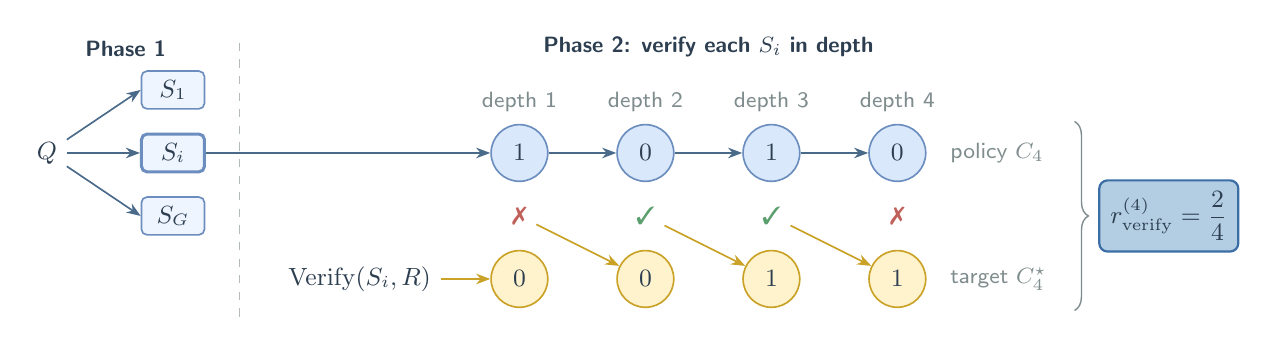
\begin{tikzpicture}[
  x=1cm, y=1cm,
  font=\sffamily\small,
  every node/.style={text=textMain},
  >={Stealth[length=1.8mm]},
  bit/.style={circle, line width=0.6pt, minimum size=0.72cm, inner sep=0pt},
  pol/.style={bit, draw=borderPrimary, fill=bgPrimary},
  tgt/.style={bit, draw=borderTarget, fill=bgHighlight},
  sol/.style={rounded corners=2pt, draw=borderPrimary, fill=bgPrimary!45, line width=0.6pt, minimum width=0.8cm, minimum height=0.48cm, inner sep=1pt},
  flow/.style={->, draw=arrowColor, line width=0.6pt},
  feed/.style={->, draw=borderTarget, line width=0.6pt},
  lab/.style={font=\sffamily\footnotesize, text=textLight},
  phase/.style={font=\sffamily\footnotesize\bfseries},
]
% Phase 1: G solutions
\node[phase, anchor=south] at (-3.2,1.1) {Phase 1};
\node (q) at (-4.2,0) {$Q$};
\node[sol] (s1) at (-2.6,0.8)  {$S_1$};
\node[sol, line width=1.1pt] (si) at (-2.6,0) {$S_i$};
\node[sol] (sg) at (-2.6,-0.8) {$S_G$};
\foreach \s in {s1,si,sg} \draw[flow] (q) -- (\s.west);
\draw[textLight!60, dashed] (-1.75,1.4) -- (-1.75,-2.1);

% Phase 2: depth-M verification of each S_i
\node[phase, anchor=south] at (4.2,1.1) {Phase 2: verify each $S_i$ in depth};
\node[anchor=east] (ver) at (0.8,-1.6) {$\operatorname{Verify}(S_i,R)$};

\foreach \d/\x/\v/\t in {1/1.8/1/0, 2/3.4/0/0, 3/5.0/1/1, 4/6.6/0/1} {
  \node[lab] at (\x,0.65) {depth \d};
  \node[pol] (p\d) at (\x,0)    {$\v$};
  \node[tgt] (t\d) at (\x,-1.6) {$\t$};
}

\node[text=badBorder] (m1) at (1.8,-0.8) {\ding{55}};
\node[text=okBorder]  (m2) at (3.4,-0.8) {\ding{51}};
\node[text=okBorder]  (m3) at (5.0,-0.8) {\ding{51}};
\node[text=badBorder] (m4) at (6.6,-0.8) {\ding{55}};

\draw[flow] (si) -- (p1);
\draw[flow] (p1) -- (p2);
\draw[flow] (p2) -- (p3);
\draw[flow] (p3) -- (p4);

\draw[feed] (ver) -- (t1);
\draw[feed] (m1) -- (t2);
\draw[feed] (m2) -- (t3);
\draw[feed] (m3) -- (t4);

% Chain names and summary score
\node[lab, anchor=west] at (7.15,0)    {policy $C_4$};
\node[lab, anchor=west] at (7.15,-1.6) {target $C_4^\star$};

\draw[textLight, line width=0.5pt, decorate, decoration={brace, amplitude=5pt}]
  (8.85,0.4) -- (8.85,-2.0);

\node[anchor=west, draw=borderAccent, fill=bgAccent, rounded corners=3pt, line width=0.8pt, inner sep=4pt]
  at (9.15,-0.8) {$r^{(4)}_{\mathrm{verify}}=\dfrac{2}{4}$};

\end{tikzpicture}

\caption{Two rollout phases. Phase~1 samples $G$ solutions to $Q$.
Phase~2 generates one verification chain of depth $M$ for each $S_i$, illustrated with $M=4$. Here $S_i$ is incorrect. Blue: policy verdicts; $v_1$ judges $S_i$, and each $v_d$ judges $v_{d-1}$. Yellow: target verdicts. Each match ({\ding{51}}/{\ding{55}}) determines the next target and supplies the current round's reward. The box reports the average accuracy across depths.}
\label{fig:depth-chain}
\end{figure}


\subsubsection{Phase 1: Solution Generation.}

For each question $Q$, the policy samples $G$ solutions $\{S_i\}_{i=1}^{G}\sim\pi_{\theta_{\mathrm{old}}}(\cdot\mid Q)$, and each receives the outcome reward $r_i=r(S_i,R)$. These rollouts are trained with $\mathcal J_{\mathrm{GRPO}}$ in \eqref{eq:grpo}, with $o_i=S_i$.


\subsubsection{Phase 2: Verification Chain Generation.}

\paragraph{Verification chain.}
For each solution $S_i$, the policy generates one verification chain of depth $M$. We describe one chain for a fixed pair $(Q,S)$ and drop the indices.

At depth $1$, the policy receives the question and the solution.
At depth $d\ge2$, it additionally receives only the previous round's
final answer $A_{d-1}$. The context is
\begin{equation}
x_d=
\begin{cases}
(Q,S), & d=1,\\
(Q,S,A_{d-1}), & d=2,\ldots,M,
\end{cases}
\end{equation}
and the policy generates a response
\begin{equation}
V_d\sim\pi_{\theta_{\mathrm{old}}}(\cdot\mid x_d),
\qquad
\bar A_d=\operatorname{ExtractAnswer}(V_d),
\end{equation}
where $\bar A_d$ is the final answer after the closing
\texttt{</think>} tag and contains a binary verdict $v_d$.
The reasoning trace inside the \texttt{<think>} tags is not
passed to subsequent rounds.

At depth $1$, the verdict judges the solution: $v_1=1$ claims that
$S$ is correct. At depth $d\ge2$, the verdict judges the previous
verdict: $v_d=1$ claims that $v_{d-1}$ is correct.
To make the final answer self-contained, we attach a running
conclusion $c_d\in\{0,1\}$ about whether $S$ is correct:
\begin{equation}
c_1=v_1,
\qquad
c_d=
\begin{cases}
c_{d-1}, & v_d=1,\\
1-c_{d-1}, & v_d=0,
\end{cases}
\quad d=2,\ldots,M.
\end{equation}
The forwarded final answer is $A_d=(\bar A_d,c_d)$.
The field $c_d$ is computed deterministically from the sampled
verdict and the previous conclusion, without using the reference
answer. It summarizes the verdict history without retaining any
earlier reasoning traces. The policy chain is
\begin{equation}
C_M=(v_1,\ldots,v_M).
\end{equation}


\paragraph{Target chain.}
The target chain $C_M^\star=(v_1^\star,\ldots,v_M^\star)$ holds the correct verdict at every depth. The first target is the phase-1 outcome reward of $S$. For $d\ge2$, the verdict $v_{d-1}$ is correct exactly when it equals its own target, so
\begin{equation}
v_1^\star=\operatorname{Verify}(S,R),
\qquad
v_d^\star=\mathds{1}\big[v_{d-1}=v_{d-1}^\star\big],
\quad d=2,\ldots,M.
\end{equation}

Let $m_d=\mathds{1}[v_d=v_d^\star]$ indicate a match at depth $d$. The recursion then reads $v_{d+1}^\star=m_d$: the target at each depth records whether the policy was right one depth earlier. The target chain is computed after the policy chain is generated and is never shown to the policy.


\paragraph{Round reward.}
Each verification round receives its own binary correctness reward:
\begin{equation}
r_d^{\mathrm{verify}}
=\mathds{1}\big[v_d=v_d^\star\big]
=m_d\in\{0,1\}.
\end{equation}
Equivalently, a verdict is correct exactly when its running
conclusion agrees with the solution's outcome:
\begin{equation}
r_d^{\mathrm{verify}}
=\mathds{1}\big[c_d=\operatorname{Verify}(S,R)\big].
\end{equation}
The average across depths is retained as a summary score:
\begin{equation}
r_{\mathrm{verify}}^{(M)}
=\frac{1}{M}\sum_{d=1}^{M}r_d^{\mathrm{verify}}\in[0,1].
\end{equation}
Training uses the individual round rewards rather than assigning
this average to every round.


\subsubsection{Training Objective.}

\paragraph{Round-level feedback.}
For solution $S_i$, let $x_{i,d}$, $V_{i,d}$, and
$r_{i,d}^{\mathrm{verify}}$ denote the context, response, and reward
at depth $d$. Each pair $(x_{i,d},V_{i,d})$ is a separate training
example. Its sampled context is held fixed during the update, and
its feedback weight is
\begin{equation}
\hat A_{i,d}^{\mathrm{verify}}
=r_{i,d}^{\mathrm{verify}}-\frac12
=
\begin{cases}
+\frac12, & v_{i,d}=v_{i,d}^\star,\\
-\frac12, & v_{i,d}\ne v_{i,d}^\star.
\end{cases}
\end{equation}
The fixed baseline $1/2$ gives positive feedback to correct rounds
and negative feedback to incorrect rounds, without comparing
different branches or depths. Phase~2 therefore uses clipped policy
gradient with a fixed baseline rather than group-normalized GRPO.

\paragraph{Verification objective.}
Let $V_{i,d,t}$ denote the $t$-th generated token of $V_{i,d}$.
The importance ratio is
\begin{equation}
\rho_{i,d,t}^{\mathrm{verify}}(\theta)=
\frac{\pi_\theta(V_{i,d,t}\mid x_{i,d},V_{i,d,<t})}
{\pi_{\theta_{\mathrm{old}}}(V_{i,d,t}\mid x_{i,d},V_{i,d,<t})}.
\end{equation}
The policy maximizes the round-level clipped objective
\begin{equation}
\label{eq:verify-objective}
\begin{aligned}
\mathcal J_{\mathrm{verify}}(\theta)
=\;&\mathbb E
\Bigg[\frac{1}{GM}\sum_{i=1}^{G}\sum_{d=1}^{M}
\frac{1}{|V_{i,d}|}\sum_{t=1}^{|V_{i,d}|}
\Big(\min\big(
\rho_{i,d,t}^{\mathrm{verify}}(\theta)
\hat A_{i,d}^{\mathrm{verify}},\\
&\qquad
\operatorname{clip}\big(
\rho_{i,d,t}^{\mathrm{verify}}(\theta),
1-\varepsilon,1+\varepsilon\big)
\hat A_{i,d}^{\mathrm{verify}}\big)
-\beta\,\mathbb D_{\mathrm{KL}}\big[
\pi_\theta\,\|\,\pi_{\mathrm{ref}}\big]\Big)\Bigg],
\end{aligned}
\end{equation}
where the expectation is over dataset questions, sampled solutions, and verification chains. The KL term is evaluated at each token's conditional context. Each round's feedback is shared by all tokens of its generated response, including its reasoning and final answer. The question, solution, previous final answer, and round instructions are masked from the loss. The deterministic conclusion field is not generated by the policy and receives no policy loss.

This objective trains each round for its own verdict accuracy on the sampled contexts; rewards from later rounds are not assigned to earlier responses. The complete verification chain is not concatenated into a single training response. The policy maximizes
\begin{equation}
\boxed{
\mathcal J(\theta)
=
\mathcal J_{\mathrm{GRPO}}(\theta)
+
\mathcal J_{\mathrm{verify}}(\theta)
}.
\end{equation}

The verification rewards evaluate binary verdicts rather than the validity of their reasoning traces. Phase~2 introduces $G\times M$ verification rounds and the same number of training examples per question.

\bibliographystyle{plainnat}
\bibliography{references}

% \section{Method}

% \subsection{Preliminaries}

% \paragraph{Policy.}
% Let $\pi_\theta$ be an autoregressive language model with parameters $\theta$. Given a question $Q$, it generates an output $o=(o_1,\ldots,o_{|o|})$ with probability
% \begin{equation}
% \pi_\theta(o\mid Q)=\prod_{t=1}^{|o|}\pi_\theta(o_t\mid Q,o_{<t}).
% \end{equation}


% \paragraph{Reinforcement learning with verifiable rewards.}
% Let $\mathcal D$ be a dataset of pairs $(Q,R)$, where $R$ is the reference answer. A rule-based verifier compares the final answer in an output $o$ with $R$ and assigns a binary reward \[r(o,R)=\operatorname{Verify}(o,R)\in\{0,1\}.\] RLVR maximizes $\mathbb E_{(Q,R)\sim\mathcal D,\;o\sim\pi_\theta(\cdot\mid Q)}\big[r(o,R)\big]$.

% \paragraph{Group relative policy optimization.}
% For each question $Q$, GRPO samples a group of $G$ outputs $\{o_i\}_{i=1}^{G}$ from the old policy $\pi_{\theta_{\mathrm{old}}}$ and computes their rewards $\{r_i\}_{i=1}^{G}$. Let $o_{i,t}$ denote the $t$-th token of $o_i$, for $t=1,\ldots,|o_i|$. All tokens of $o_i$ share the same group-normalized advantage
% \begin{equation}
% \hat A_{i,t}=
% \frac{r_i-\operatorname{mean}\big(\{r_j\}_{j=1}^{G}\big)}
% {\operatorname{std}\big(\{r_j\}_{j=1}^{G}\big)}.
% \end{equation}

% The policy is updated by maximizing
% \begin{equation}
% \label{eq:grpo}
% \begin{aligned}
% \mathcal J_{\mathrm{GRPO}}(\theta)
% =\;&\mathbb E_{(Q,R)\sim\mathcal D,\;
% \{o_i\}_{i=1}^{G}\sim\pi_{\theta_{\mathrm{old}}}(\cdot\mid Q)}
% \Bigg[\frac{1}{G}\sum_{i=1}^{G}\frac{1}{|o_i|}\sum_{t=1}^{|o_i|}
% \Big(\min\big(\rho_{i,t}(\theta)\hat A_{i,t},\\
% &\qquad\operatorname{clip}\big(\rho_{i,t}(\theta),1-\varepsilon,1+\varepsilon\big)\hat A_{i,t}\big)
% -\beta\,\mathbb D_{\mathrm{KL}}\big[\pi_\theta\,\|\,\pi_{\mathrm{ref}}\big]\Big)\Bigg],
% \end{aligned}
% \end{equation}
% where
% \begin{equation}
% \rho_{i,t}(\theta)=
% \frac{\pi_\theta(o_{i,t}\mid Q,o_{i,<t})}
% {\pi_{\theta_{\mathrm{old}}}(o_{i,t}\mid Q,o_{i,<t})}
% \end{equation}

% is the importance ratio, $\varepsilon$ is the clipping range, and $\beta$ weights the KL penalty toward a frozen reference policy $\pi_{\mathrm{ref}}$.

% \subsection{Proposed Idea: Scaling Verification Depth}

% Each training step has two rollout phases (\cref{fig:depth-chain}).
% Phase~1 is the standard GRPO rollout: the policy samples $G$ solutions
% to a question. Phase~2 scales verification in depth: the policy
% generates one verification chain of $M$ sequential rounds for each
% solution, where $M$ denotes the verification depth.
% Both phases sample from $\pi_{\theta_{\mathrm{old}}}$ and are
% optimized in the same update.

% \begin{figure}[t]
% \centering
% \begin{tikzpicture}[
%   x=1cm, y=1cm,
%   font=\sffamily\small,
%   every node/.style={text=textMain},
%   >={Stealth[length=1.8mm]},
%   bit/.style={circle, line width=0.6pt, minimum size=0.72cm, inner sep=0pt},
%   pol/.style={bit, draw=borderPrimary, fill=bgPrimary},
%   tgt/.style={bit, draw=borderTarget, fill=bgHighlight},
%   sol/.style={rounded corners=2pt, draw=borderPrimary, fill=bgPrimary!45, line width=0.6pt, minimum width=0.8cm, minimum height=0.48cm, inner sep=1pt},
%   flow/.style={->, draw=arrowColor, line width=0.6pt},
%   feed/.style={->, draw=borderTarget, line width=0.6pt},
%   lab/.style={font=\sffamily\footnotesize, text=textLight},
%   phase/.style={font=\sffamily\footnotesize\bfseries},
% ]
% % Phase 1: G solutions
% \node[phase, anchor=south] at (-3.2,1.1) {Phase 1};
% \node (q) at (-4.2,0) {$Q$};
% \node[sol] (s1) at (-2.6,0.8)  {$S_1$};
% \node[sol, line width=1.1pt] (si) at (-2.6,0) {$S_i$};
% \node[sol] (sg) at (-2.6,-0.8) {$S_G$};
% \foreach \s in {s1,si,sg} \draw[flow] (q) -- (\s.west);
% \draw[textLight!60, dashed] (-1.75,1.4) -- (-1.75,-2.1);

% % Phase 2: depth-M verification of each S_i
% \node[phase, anchor=south] at (4.2,1.1) {Phase 2: verify each $S_i$ in depth};
% \node[anchor=east] (ver) at (0.8,-1.6) {$\operatorname{Verify}(S_i,R)$};

% \foreach \d/\x/\v/\t in {1/1.8/1/0, 2/3.4/0/0, 3/5.0/1/1, 4/6.6/0/1} {
%   \node[lab] at (\x,0.65) {depth \d};
%   \node[pol] (p\d) at (\x,0)    {$\v$};
%   \node[tgt] (t\d) at (\x,-1.6) {$\t$};
% }

% \node[text=badBorder] (m1) at (1.8,-0.8) {\ding{55}};
% \node[text=okBorder]  (m2) at (3.4,-0.8) {\ding{51}};
% \node[text=okBorder]  (m3) at (5.0,-0.8) {\ding{51}};
% \node[text=badBorder] (m4) at (6.6,-0.8) {\ding{55}};

% \draw[flow] (si) -- (p1);
% \draw[flow] (p1) -- (p2);
% \draw[flow] (p2) -- (p3);
% \draw[flow] (p3) -- (p4);

% \draw[feed] (ver) -- (t1);
% \draw[feed] (m1) -- (t2);
% \draw[feed] (m2) -- (t3);
% \draw[feed] (m3) -- (t4);

% % Chain names and reward
% \node[lab, anchor=west] at (7.15,0)    {policy $C_4$};
% \node[lab, anchor=west] at (7.15,-1.6) {target $C_4^\star$};

% \draw[textLight, line width=0.5pt, decorate, decoration={brace, amplitude=5pt}]
%   (8.85,0.4) -- (8.85,-2.0);

% \node[anchor=west, draw=borderAccent, fill=bgAccent, rounded corners=3pt, line width=0.8pt, inner sep=4pt]
%   at (9.15,-0.8) {$r^{(4)}_{\mathrm{verify}}=\dfrac{2}{4}$};

% \end{tikzpicture}

% \caption{Two rollout phases. Phase~1 samples $G$ solutions to $Q$.
% Phase~2 generates one verification chain of depth $M$ for each $S_i$, illustrated with $M=4$. Here $S_i$ is incorrect. Blue: policy verdicts; $v_1$ judges $S_i$, and each $v_d$ judges $v_{d-1}$. Yellow: target verdicts. Each match ({\ding{51}}/{\ding{55}}) determines the next target.}
% \label{fig:depth-chain}
% \end{figure}


% \subsubsection{Phase 1: Solution Generation.}

% For each question $Q$, the policy samples $G$ solutions $\{S_i\}_{i=1}^{G}\sim\pi_{\theta_{\mathrm{old}}}(\cdot\mid Q)$, and each receives the outcome reward $r_i=r(S_i,R)$. These rollouts are trained with $\mathcal J_{\mathrm{GRPO}}$ in \eqref{eq:grpo}, with $o_i=S_i$.


% \subsubsection{Phase 2: Verification Chain Generation.}

% \paragraph{Verification chain.}
% For each solution $S_i$, the policy generates one verification chain of depth $M$. We describe one chain for a fixed pair $(Q,S)$ and drop the indices.

% At depth $d\in\{1,\ldots,M\}$, the policy receives the question, the solution, and all earlier rounds $V_{<d}=(V_1,\ldots,V_{d-1})$, and generates
% \begin{equation}
% V_d=(E_d,v_d)
% \sim\pi_{\theta_{\mathrm{old}}}(\cdot\mid Q,S,V_{<d}),
% \end{equation}

% where $E_d$ is a written analysis and $v_d\in\{0,1\}$ is a verdict. At depth $1$, the verdict judges the solution: $v_1=1$ claims that $S$ is correct. At depth $d\ge 2$, the verdict judges the previous verdict: $v_d=1$ claims that $v_{d-1}$ is correct. The policy chain is:
% \begin{equation}
% C_M=(v_1,\ldots,v_M).
% \end{equation}


% \paragraph{Target chain.}
% The target chain $C_M^\star=(v_1^\star,\ldots,v_M^\star)$ holds the correct verdict at every depth. The first target is the phase-1 outcome reward of $S$. For $d\ge 2$, the verdict $v_{d-1}$ is correct exactly when it equals its own target, so
% \begin{equation}
% v_1^\star=\operatorname{Verify}(S,R),
% \qquad
% v_d^\star=\mathds{1}\big[v_{d-1}=v_{d-1}^\star\big],
% \quad d=2,\ldots,M.
% \end{equation}


% Let $m_d=\mathds{1}[v_d=v_d^\star]$ indicate a match at depth $d$. The recursion then reads $v_{d+1}^\star=m_d$: the target at each depth records whether the policy was right one depth earlier. The target chain is computed after the policy chain is generated and is never shown to the policy.

% % The target chain is built from the policy chain, not fixed in advance. A fixed target $(v_1^\star,1,\ldots,1)$ would reward the policy for endorsing a wrong $v_1$. Under the recursive target, a wrong verdict at depth $d$ sets $v_{d+1}^\star=0$, so the policy is rewarded for detecting the error and penalized for rejecting a correct verdict.


% \paragraph{Depth reward.}
% The depth reward is the fraction of depths at which the two chains agree:
% \begin{equation}
% r_{\mathrm{verify}}^{(M)}
% =\frac{1}{M}\sum_{d=1}^{M}
% \mathds{1}\big[v_d=v_d^\star\big]
% =\frac{1}{M}\sum_{d=1}^{M}m_d\in[0,1].
% \end{equation}

% Dividing by $M$ keeps the reward in the same range at every depth.


% \subsubsection{Training Objective.}

% Let $r_i^{\mathrm{verify}}$ be the depth reward of the verification chain for solution $S_i$. Advantages are normalized across the $G$ verification chains associated with each question:
% \begin{equation}
% \hat A_i^{\mathrm{verify}}=
% \frac{
% r_i^{\mathrm{verify}}
% -\operatorname{mean}\big(
% \{r_j^{\mathrm{verify}}\}_{j=1}^{G}
% \big)
% }{
% \operatorname{std}\big(
% \{r_j^{\mathrm{verify}}\}_{j=1}^{G}
% \big)+\epsilon_{\mathrm{norm}}
% },
% \end{equation}

% where $\epsilon_{\mathrm{norm}}>0$ is a small constant for numerical stability.

% Each advantage is shared by all generated tokens of its verification chain, including the analyses and verdicts of all $M$ rounds. The question, the solution, and the round prompts are masked. Applying the clipped objective in \eqref{eq:grpo} to these chains with advantages $\hat A_i^{\mathrm{verify}}$ gives $\mathcal J_{\mathrm{verify}}$. The policy maximizes
% \begin{equation} 
% \boxed{
% \mathcal J(\theta)
% =
% \mathcal J_{\mathrm{GRPO}}(\theta)
% +
% \mathcal J_{\mathrm{verify}}(\theta)
% }
% \end{equation}



% The depth reward evaluates binary verdicts rather than the validity of their written analyses. Phase~2 introduces $G \times M$ verification rounds per question.

% \bibliographystyle{plainnat}
% \bibliography{references}



\end{document}